\section{System architecture and design}
This section will describe the architecture and the design process. We start of by presenting the most architectural significant requirements. Then we address what tactics and patterns used to fulfill these, before discussing the design process. We round up with architectural views and a rationale. Figure ~\ref{fig:overall_architecture} is a brief sketch of the final architecture.

\begin{figure}[H]
\centering
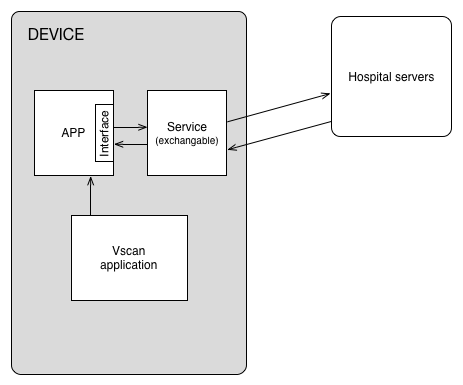
\includegraphics[scale=0.7]{img/system_arch.png}
\caption{Final system architecture}
\label{fig:overall_architecture}
\end{figure}

\newpage

%%%%%%%%%%%%%%%%%%%% NY SUBSECTION %%%%%%%%%%%%%%%%%%%%

\subsection{Architectural Significant Requirements}
Combining the requirements and business goals, the group wanted to create a secure application that was easy to use whilst reducing the cost of modifying it. While usability was important, it would not be as significant to the architecture as security and interoperability turned out to be. How the architecture reflects the functional requirements is addressed in section \ref{architectualRationale}. Table \ref{asrtable} shows the architectural significant requirements.

%Tabell for functional requirements
\begin{table}[H]

\renewcommand{\arraystretch}{1.2}
\captionof{table}{Architectural significant requirements}
\label{asrtable}
\begin{tabular}{|p{3cm}|p{9cm}|}
\hline
\textbf{FR\#} & \begin{tabular}[c]{@{}l@{}}
\textbf{Description}
\end{tabular} \\ \hline

3 & \begin{tabular}[c]{@{}l@{}}
The application need to allow doctors to authenticate\\ with the EMR-system
\end{tabular} \\ \hline

4 & \begin{tabular}[c]{@{}l@{}}
The application must be able to identify patients \\
based on SSN
\end{tabular} \\ \hline

5 & \begin{tabular}[c]{@{}l@{}}
The application need to be able to upload images to \\
the hospital servers
\end{tabular} \\ \hline

10 & \begin{tabular}[c]{@{}l@{}}
The application must not display sensitive information\\ 
if the application is in offline mode
\end{tabular} \\ \hline

12 & \begin{tabular}[c]{@{}l@{}}
The application must auto-close and/or auto-log out \\ after a  
given time interval 
\end{tabular}\\ \hline

\end{tabular}
\end{table}



\paragraph*{Interoperability}
%Having a modular product will impact on the design of the architecture.  Thearchitectural design must allow for several modules that have low couplingand high cohesion, so that it is easy and cost efective to customize one partof the system while the rest stays the same.
Interoperability is an important quality attribute for the application, as one of its main features involves communicating with an external hospital information system. 


\paragraph*{Security}
In order to properly secure the application, security has to be built in to the architecture. It is important to restrict access as well as securing resources.


%%%%%%%%%%%%%%%%%%%% NY SUBSECTION %%%%%%%%%%%%%%%%%%%%

\newpage

\subsection{Tactics}
In the following section we will describe the tactics used in order for the architecture to meet the quality requirements.

\subsubsection{Security}
\label{architecturesecurity}
Through research, it was confirmed that the back-end of the hospital information systems used a lot of security tactics, ranging from detecting attacks to recovering from them. Because of this, it was decided to focus on tactics for resisting attacks to secure the application. How this decision opens for potential threats is reflected upon in section \ref{productEval}.

\paragraph*{Authentication}
Users should provide evidence that they actually are who they claim to be. This is usually done through usernames and passwords.

\paragraph*{Encrypt data}
Data should be protected from unauthorized access. Confidentiality can be achieved by applying encryption to both data and communication.

\subsubsection{Interoperability}
The application need to communicate with a hospital information system. This is done through a service acting as an intermediary between the application and the server.

\paragraph*{Locate}
The locate tactic is about the fact that the systems involved should know about each other. 

\paragraph*{Manage interfaces}
The involved systems needs to understand each other in order to exchange information.

%The basic approach to reducing the cost of modifying responsibilities is to transform the architecture by splitting the responsibility into two portions based on the specific change to be made (Bachmann et al. 2007) \cite{1504552}.

%To accommodate for the quality attributes presented in \ref{modularityQA}, we chose to focus on increasing cohesion and reduce coupling. This, combined with carefully defining responsibility for different modules, ultimately led to the decision to separate the application into a on-device Android service and a normal GUI application, which is specified in section \ref{serviceDescription}.

%\paragraph*{Encapsulation}
%Objects should be encapsulated. The object’s functionality should be exposed to the rest of the program via its public methods.

%\paragraph*{Use an Intermediary}
%If an object depends on functionality from a complex service, an intermediary layer with a simplified interface should be used.

%\paragraph*{Restrict dependencies}
%An object should not reference other objects unless they are immediately relevant.

%\paragraph*{Split responsibility}
%Making one module of a system be responsible for a well defined task and thereby splitting the responsibility reduces the cost of particular changes.


%%%%%%%%%%%%%%%%%%%% NY SUBSECTION %%%%%%%%%%%%%%%%%%%%

\subsection{Patterns}
This section contains an overview of the architectural- and design patterns used in the application. 


\subsubsection{Singleton}
\label{singletonArc}
The \emph{singleton} pattern is a design pattern that is used in order to prohibit the instantiation of more than one instance of a class \cite{softwarearchitecture}. The idea is that instead of letting other classes access the constructor and create new instances of the class, the constructor is made private. Everything has to go through another (static) method, typically called \emph{getInstance(...)}, which handles access to the class. In the implementation, we have utilized the singleton pattern in the database helper class. Section \ref{databaseImp} will go over the implementation in greater detail.

\subsubsection{ViewHolder}
\label{viewholderArc}
The ViewHolder pattern is an Android specific design pattern used to increase performance in \emph{ListViews}. The pattern is crucial to implement when dealing with large lists to avoid bad performance. A detailed explanation of how the patterns works, as well as implementation details can be found in section \ref{viewholderImp}.


\subsubsection{MVC}
The Model-View-Controller architectural pattern (MVC) divides the architecture of an application into three components. The model contains the core functionality and data, while controllers handle user input and views display information. This pattern reduce coupling by enforcing encapsulation and makes it easier to implement an intermediary layer where needed. This ultimately makes it easier to make modifications, both to logical components as well as to the user interface. From a security perspective, the developer got more control over the data, as it resides in the model.


%%%%%%%%%%%%%%%%%%%% NY SUBSECTION %%%%%%%%%%%%%%%%%%%%


\subsection{Design Process}
In the start of the development process the group did not have access to a lot of technical information from the hospitals and their information systems. While waiting for a response, the group started the development of the user interface as this did not require much information from others than the customer. Almost all the application's functionality was already in place before the server connection was implemented.

\subsubsection{Offline Mode}
One of the additional features the customer requested was the ability to use the application without a network, or away from the hospital. This would enable the user to conduct examinations on home visits and remote locations, store all the data on the device and upload it when the application gets network access again.

The group designed offline mode to work in such a way that once network connection is lost, the application automatically enters offline mode. Here, sensitive data is stripped because it is not possible to authenticate the user while offline.

During the later part of the development period, we changed how the application decrypts the database. This change cascaded in such a way that the current implementation of offline mode stopped working. Further information about this event is found in section \ref{evaloffline}.


\subsubsection{Service}
\label{serviceDescription}

While the initial plan was to communicate with a “XML package”, the new approach included creating a separate Android Service \cite{android_service}. Research showed the code needed to do the actual communication with the hospital servers was trivial for a developer with knowledge about the system in question. However the code for connecting to one system was unique to another. This led to the conclusion that the service should be standardized in such a way that it could easily be implemented. The service should provide two tasks to the application; identifying a patient, and uploading images and examination data. An interface was defined so that developers would know what data to expect, and what to return to the application. A template for the service was also developed, and is (together with the interface) documented in the developer guide in the Appendix \ref{devmanual}.

To make this interface work, the group started working with AIDL (Android Interface Definition Language). AIDL allows the programmer to define a general interface to communicate with services without defining the exact service. This way it was possible to choose which service to use, and more services could be made later to support new standards and servers.

The content of the messages exchanged between the service and the application had to be decided. Based on information gathered from the industry, the group learned that this had to include name and SSN. In addition, Norwegian systems required department credentials in order to execute correctly (more information in section \ref{exsol}).

The application was therefore changed to support this feature, so that the technical user would be prompted with department username and password during first time set up. By prompting the user in such a way, the application also maintained a level of diversity in regards to the goal of making the application work anywhere, because the user has the option of entering his own credentials, should the hospital not operate with a department user policy.

It was early discovered that the Vscan was able to record video as well as images. The application was therefore designed with this in mind, and there is intentionally no restrictions hindering the user in uploading other files than images.

Overall, the new architecture worked exceptionally well, and also allowed for some new features. As before, when the application only was to upload data to a hospital server by a doctor, the application could now also be tailored to other medical practitioners by changing the service. This way, radiologists who did not wish to upload examinations to a shared multimedia storage, could for example be given a version where the service uploaded DICOM files to their conventional PACS.

When the service system was in place, it was decided to create an example service. Initially, the group intended to create a service that communicated with a DIPS mockup server, making it as realistic as possible. Through contacts in the industry, access to a DIPS BizTalk server in Oslo was acquired. We encountered several, both technical and practical, problems when trying to implement this service using the HL7 CDA R2 messaging standard. Because these issues were not resolved, we have not included the design and implementation details of the DIPS service in this report. However, these details can be found in Appendix \ref{biztalk}. 

As a backup plan we designed a really simple service, just to illustrate that our architecture worked. This service would query an SQL server for patient data, and uploading the image data to an SFTP server. This service was quickly implemented, and it communicated with the application as intended.

\noindent
Because Vscan Gateway, described in section \ref{vscan} of the report, was able to generate an examination report as a PDF, the group decided that the backup service should do the same. To build further on the proof of concept, the service never stores any data to disk, including the PDF which is generated in memory. An example report generated by the backup service, can be found in Appendix \ref{dummyServiceReport}.


\subsubsection{Settings}
The choice to use an XML file to setup the application was one of the first features that was implemented, and never actually changed. The reason for this is that it would make it easier for technical users to set up several devices at the same time, as well as providing the rest of the system a modifiable list of settings that could be expanded as more parameters were needed. The XML parser was originally implemented to work with both the package system and the settings. When the package system idea was scrapped, only the settings utilized the parser.


%%%%%%%%%%%%%%%%%%%% NY SUBSECTION %%%%%%%%%%%%%%%%%%%%


\subsection{Architectural views}
We considered the developer and the customer to be the two stakeholders that had to understand the structure of the application. Based on this, a development view and process view were created to help these groups of stakeholders get an understanding of the application.

%In order to achieve this, a component and connector view and a allocation view were created for making stakeholders understand the concepts  

\newpage

\subsubsection{Development view}
The development view illustrates the system from a developers perspective \cite{softwarearchitecture}. The emphasis is on the layers the system consists of, and serves the purpose of giving developers of getting an overview of the system. A three-layer structure is used in order to separate the key parts of the application. These are the graphical user interface, the application logic, the service and the underlying operating system (Android SDK).

\begin{figure}[H]
\centering
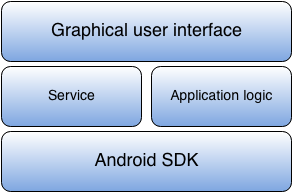
\includegraphics[scale=0.7]{img/development_view.png}
\caption{Development view}
\label{fig:development_view}
\end{figure}


\subsubsection{Process view}
The process view focuses on representing the flow of the application in a way that is easily understandable for all the stakeholders. It shows how the application combine different actions into a seamless process. As the application starts, the user has to make a decision. This happens with the "Login"-view, and there are three possible outcomes: either the user is able to authenticate to the hospital server, or the application in offline mode, where all existing data is anonymized. The only possible operation in this mode is to add new examinations or view the images of old ones. The third possible entry point is as a technical user. This option is protected by a password. The rest of the process is illustrated in the flowchart below.

%Deprecated!
\begin{sidewaysfigure}
    \centering
    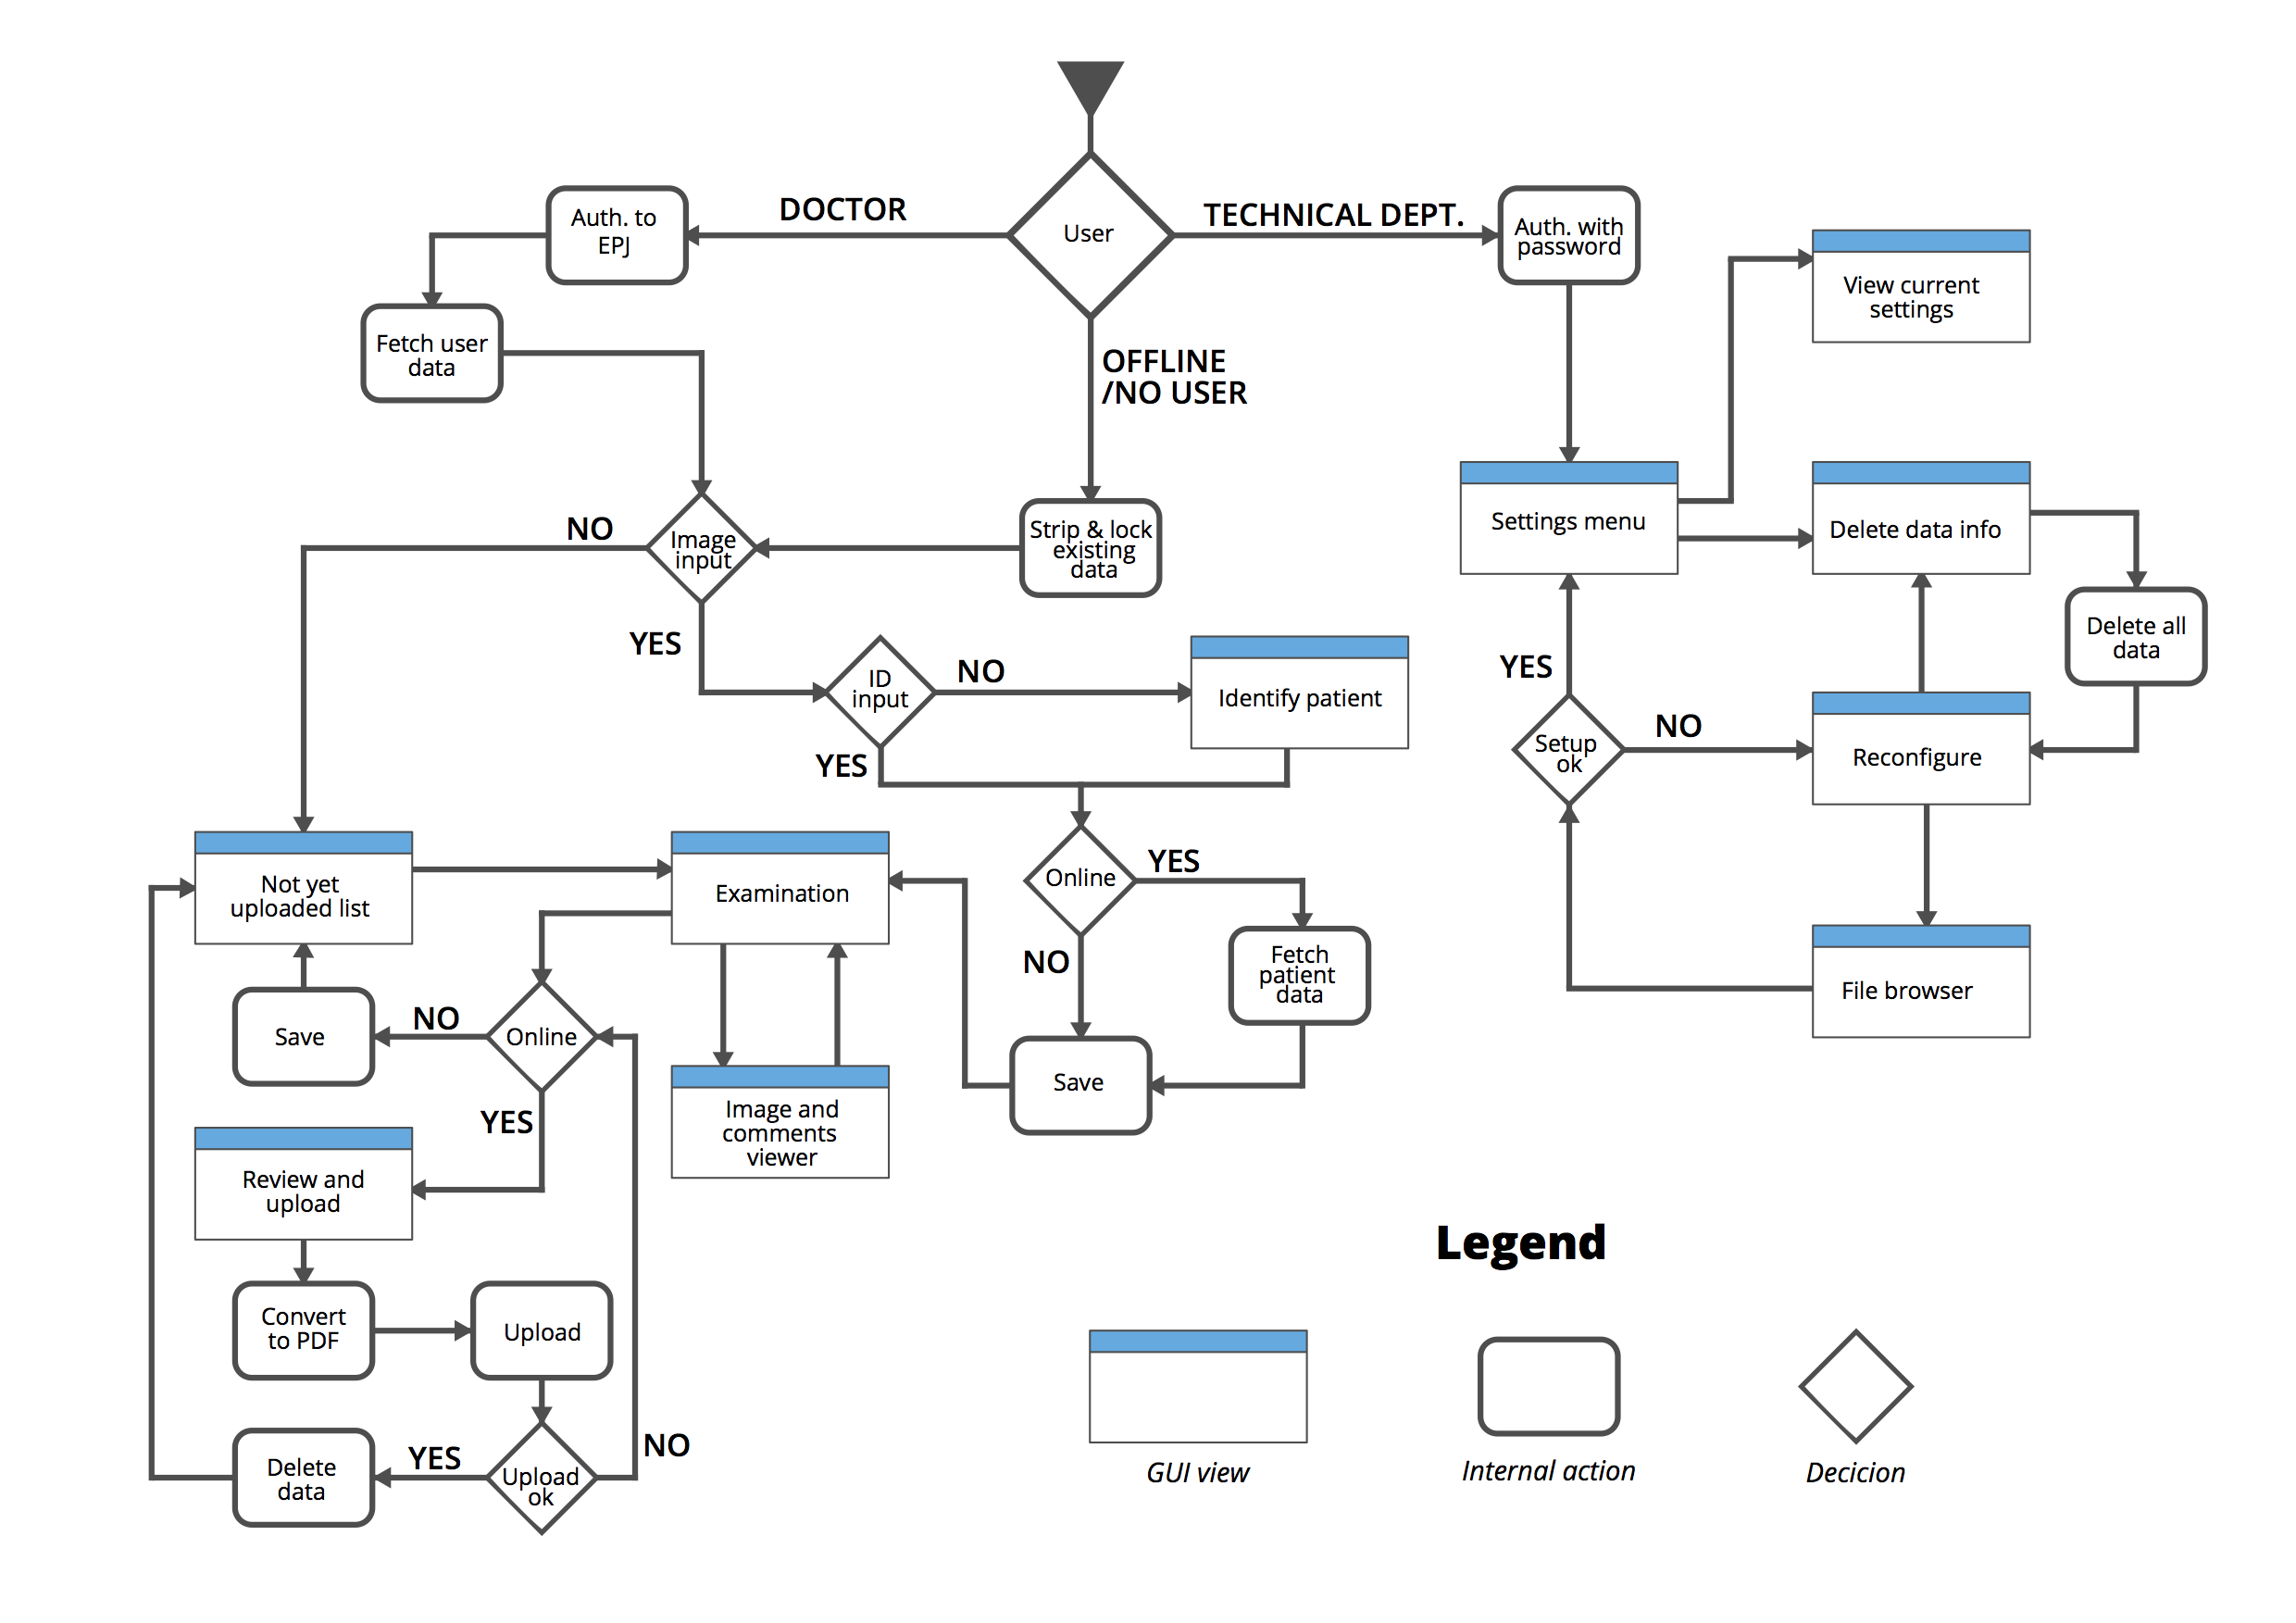
\includegraphics[scale=0.45]{img/flowchart.png}
    \caption{Process view of the application}
    \label{fig:flowchart}
\end{sidewaysfigure}
\newpage


%%%%%%%%%%%%%%%%%%%% NY SUBSECTION %%%%%%%%%%%%%%%%%%%%


\subsection{Architectural Rationale}
\label{architectualRationale}
The functional requirements and quality requirements are designed to reflect the architectural drivers and the interests of the stakeholders. In this section, how the architecture fulfills these requirements will be described.

\subsubsection{Functional Requirements}
First of all, the application needs to allow doctors to authenticate to the hospital servers. This is fulfilled by using Active Directory as an authentication service.

The functional requirement describing how the application must be able to identify patients based on SSN, is fulfilled by sending the information to the Android service. This takes care of communication with the respective hospital system.

To fulfill the requirement about being able to upload images to the hospital servers the application lets the Android service take care of this too.

\subsubsection{Quality Requirements}

\paragraph*{INT1 \& INT2 - Different services, same functionality}
By separating the architecture into one application and one service, we fulfilled both of the interoperability requirements. Through the AIDL interface, it is possible to implement new versions of the service. By replacing the service the same application can communicate with different hospital systems. At the same time this enables the main application to stay the same regardless of what service is actually used.

\paragraph*{SEC1 - Encrypted data}
The application fulfills the quality requirement regarding encrypted data with the use of SQLCipher - encrypting the database. This is done by encrypting the whole database file, and no additional concerns regarding architecture was needed.

\paragraph*{SEC2 - Data should not be able to leave the application}
With the model-view-controller approach, we got better control of the the data as it resides in the model instead of being scattered around.